% !TEX root =  ../Dissertation.tex

\chapter{Design}

\section{Methodology}
\begin{figure}[h] % 'h' means 'here' - places the figure where it's defined
    \centering
    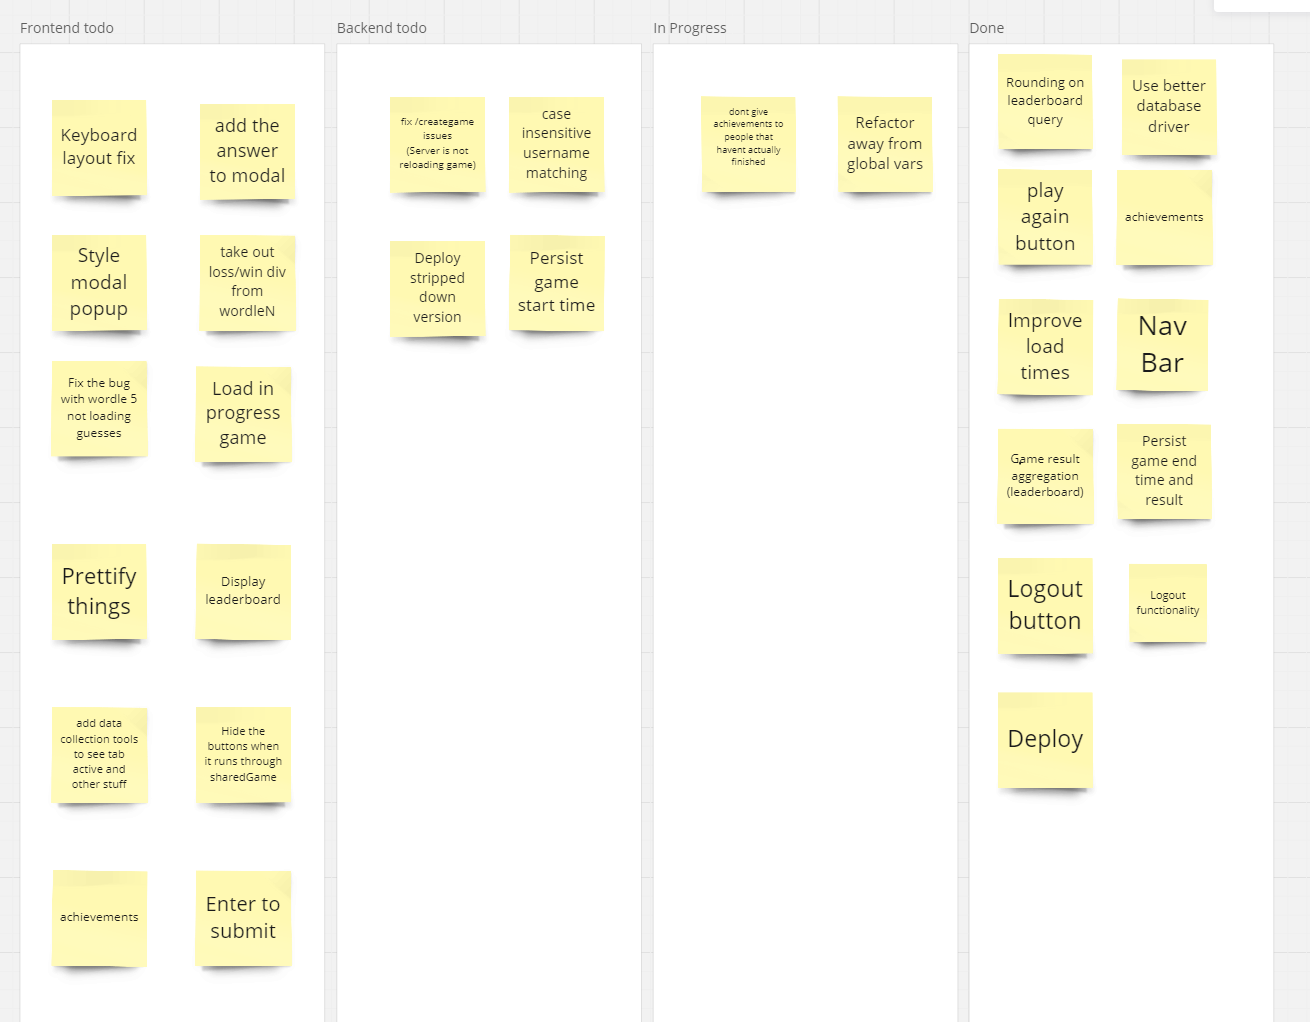
\includegraphics[width=\textwidth]{Kanban_Board.png} % Replace with your image file
    \caption{Kanban Board partway through production}
    \label{fig:example}
\end{figure}
While development was only finished by one person, it was pertinent to have a methodology to use while components were in development. For this, a Kanban approach was used,\cite{Toyota2021} using a web application called Miro. A project board with an essential to-do, in-progress, and finished workflow was created.\cite{Miro2024} The workflow limit was two, so there would only be that many in the in-progress swim lane simultaneously. 

This approach allowed the ability to focus on vertical slices of the product each time, which works in tandem with React's component approach to building functioning web applications and creating vertical slices of incremental value.\cite{Sarrion2023}

\section{Goals and Approach}
A participant in the later experiment was interviewed before development was started, particularly on the web application's retention techniques. The main goal of the interview was to understand what would make players want to return to a Wordle application and what made them leave in the first place. It was also important to identify which user retention techniques would feel most natural to the user to be incorporated into a daily game web application.

The interviewee was previously an avid player of Wordle when it was first released but had slowly stopped playing. They reasoned that they had gotten ‘tired’ of playing the same thing daily, especially when they found that they would always find the answer. They also found that after a certain amount of time, people stopped sending the emoji grid, showing users their daily score. 

While it is helpful to get ideas from users, sometimes a web application implements a feature that a user was unaware they would want until it was implemented. The user was presented with a list of retention techniques and asked to select their preferred option.

Different retention techniques, such as a daily reward schedule, were considered, where consistent logins would grant rewards. For Wordle, this would take the form of a user logging in three days in a row, and the third day would give them the first letter of their first guess, allowing for a higher chance of a better score. The user was against this idea as they already found Wordle too easy and thought that this would apply too much pressure for them to log in daily. 

The user thought the leaderboard was ideal, as it eliminated sharing the emoji grid and allowed users to see their average score throughout the day. Having achievements to strive for was also noted to be appropriate and unintrusive, while still being an enjoyable way to want to play more.

The Gauntlet now also uses increased functionality, such as longer-length words to guess and the ability to share your previous word with a user. These were not decided upon until later, but after a brief conversation, the user deemed them both appropriate additions. 

With the information collected in the literature review and initial conversations with a participant regarding additional retention techniques, that are both appropriate and interesting, forward progress can be made with several goals established.

Emphasizing the social aspect presents a compelling approach, as this was brought up when asking a user as well as in the scholarship. This will take the form of a leaderboard, meaning that the user will not have to go out of their way to send their ‘emoji grid’ to other users. It will also add a competitive nature to give something for users to strive for. Introducing achievements has proven to be a suitable strategy, as achievements are a key method for retaining users, and they are unlikely to continue using the application if they do not feel adequately challenged. The increased functionality will give users more reason to return to the web application while increasing the challenge with the WordleN feature. A new method of sociability will also be tested, with the ability to share a user's previous game. This will encourage users to talk and share about the web application, leading to increased retention over a longer period. This will take the form of the following design goals for each component:

\subsection{Wordle}
First and foremost, for the web application to be able to test these retention techniques, we must have a game to test it around. Wordle is the clear choice as it is the originator and the site that popularised the daily game genre of web applications. A level of parity between The Gauntlet and Wordle's main features will be attempted. Since Wordle is already a popular game, this will ensure that the quality of a new theoretical game that could be created doesn't influence users' enjoyment of the web application. It will be asked if people were tired of Wordle before using the web app to determine if that influences how much they played. The only core difference between The Gauntlet and Wordle will be that people can play more than one game daily.

\subsection{Leaderboard}
Instead of having users share their scores on a third-party social media platform such as Twitter, which, while excellent for player acquisition, has little effect on user retention. The web application will implement a Leaderboard page where users will be ranked primarily on their average Wordle score. If players have the same average score, the ranking will be decided based on their average time spent on completing a Wordle puzzle. 

\subsection{Achievements}
The web application will also implement an achievement system. While the achievements are somewhat rudimentary, a fleshed-out version of the system can be implemented, with further time invested in more features that will reward players for engaging with all aspects of the web application. Users will be able to see their incomplete achievements, which will give them something to aspire to and increase their drive to continue engaging with the game.

\subsection{Share}
As discussed in the Literature Review, the social aspect of a game is highly beneficial for user retention. The ‘emoji grid’ was highly successful for the original Wordle game, as this relates much more to user acquisition than user retention and is, therefore, outside this paper's scope. This social aspect helps with the competition that can break out due to having a leaderboard, but having something more engaging between users may be helpful. An alternate solution is available to this web application as it is not constrained by the limit of one game per day that Wordle has placed upon itself. Instead of sending your result to another user, send the word you just finished playing. A ‘Share’ button will add this feature to copy a clipboard link after your game. You can share this link with another person, allowing them to start a new game that uses the same word you just played within your current game.

\subsection{WordleN}
Increased functionality also benefits user retention. The apparent expansion to Wordle is an increased word length. While this does come with complications and some changes to the rules, such as an increased number of guesses, it is also imperative to have functionality with all the other components I have described.

\section{Functional and Non-Functional Requirements}
The functional and non-functional requirements outlined in the Requirements section are essential, detailed specifications that define the expected behaviour and performance of the application. These requirements ensure that the development team and the stakeholders understand what the application must achieve by the end of its development cycle.

Each requirement has been carefully articulated to specify the actions and outcomes the application must support within the key functional areas described (such as Wordle Game Mechanics, Achievements, Leaderboards, and Sharing Features). For instance, the Wordle component must allow users to guess words and receive immediate feedback, while the Achievement system must accurately update and display user progress.

Additionally, non-functional requirements such as performance, security, and usability are documented to ensure the application meets its functional goals and delivers a reliable, secure, and user-friendly experience. These requirements include specifications like response times, data encryption, and accessibility standards, which are critical to the overall quality and success of the application.

Documenting these functional and non-functional requirements is imperative, as it establishes a mutual agreement between the developers and stakeholders. This clarity facilitates smoother development, reduces the risk of misunderstandings, and ensures that the final product aligns with the stakeholders' expectations. As development progresses, all stakeholders will continually review and refine these requirements to adapt to evolving needs or insights.

\clearpage
\subsection{Functional Requirements}
\begin{tabularx}{\textwidth}{|l|X|c|}
\hline
\textbf{Type} & \textbf{Requirement} & \textbf{Importance} \\
\hline
\endfirsthead

\hline
\textbf{Type} & \textbf{Requirement} & \textbf{Importance} \\
\hline
\endhead

\hline
\multicolumn{3}{|r|}{\small\textit{Continued on next page}} \\
\hline
\endfoot

\hline
\endlastfoot
\hline
Wordle & Let a user guess a five-letter word & M \\
\hline
Wordle & Have the Keyboard change each letter to the correct state & M \\
\hline
Wordle & Have each letter change to the correct state & M \\
\hline
Wordle & Have the end game modal box show after a loss/win & S \\
\hline
Wordle & Have the game saved after each finished game & S \\
\hline
Wordle & Have words be checked against a comprehensive English dictionary & S \\
\hline
Achievements & Be updated after each game & M \\
\hline
Achievements & Have the page display the correct achievements for each user & M \\
\hline
Achievements & Have an option to suggest achievements & C \\
\hline
Keyboard & Layout should match the qwerty layout & S \\
\hline
Achievements & Have the user only receive the achievement when they have completed the task & M \\
\hline
Achievements & Ensure users only have their own achievements displayed & M \\
\hline
Achievements & If new achievements are released, progress is backdated from the database & M \\
\hline
Achievements & Receive a pop-up that notifies the user when they have been awarded an achievement & S \\
\hline
Leaderboards & Have accurate information on the score of each user & M \\
\hline
Leaderboards & Contain the score and rank of all users & M \\
\hline
Leaderboards & Should split leaderboards for each game mode & S \\
\hline
Leaderboards & Add average time to the leaderboard as a tiebreaker for users with the same average score & C \\
\hline
Share & Add a link to a clipboard containing the UUID of the shared game & M \\
\hline
Share & When the link is used it takes a user to Wordle with the correct answer & M \\
\hline
\end{tabularx}


\subsection{Non-Functional Requirements}
\begin{tabularx}{\textwidth}{|l|X|c|}
\hline
\textbf{ID} & \textbf{Requirement} & \textbf{Importance} \\
\hline
NFR 1 & Have the guess parsed in less than 500ms & M \\
\hline
NFR 1.1 & Have a load time of less than 500ms & M \\
\hline
NFR 1.2 & Ensure all pages load within 1 second under normal conditions. & M \\
\hline
NFR 1.3 & Handle up to 10 concurrent transactions per second during peak usage without noticeable lag. & M \\
\hline
NFR 1.4 & Achievements should be updated and visible to the user within 2 seconds of being earned. & M \\
\hline
NFR 1.5 & Load the leaderboard in under 500ms & M \\
\hline
NFR 1.6 & Optimize the system to minimize delays in unlocking and notification delivery & S \\
\hline
NFR 1.7 & Have the app be optimized to run efficiently on devices with limited resources (e.g., older smartphones). & S \\
\hline
NFR 1.8 & Not add load time to the Wordle webpage & S \\
\hline
NFR 2 & Have sensitive data, such as user credentials, be encrypted using JWT. & M \\
\hline
NFR 2.1 & Implement basic password protection for user accounts & M \\
\hline
NFR 2.2 & Ensure that user data is only accessible by the individual user and administrators with explicit permissions. & M \\
\hline
NFR 3 & Have a simple, clean interface that is easy to navigate for users of varying technical skill levels. & M \\
\hline
NFR 3.1 & Be accessible to all users, supporting basic accessibility features like text resizing and screen reader compatibility. & S \\
\hline
NFR 3.2 & Ensure the app is fully functional on Android and iOS devices, with a responsive design for various screen sizes. & S \\
\hline
NFR 4.1 & Handle errors gracefully, displaying user-friendly messages and logging errors for later review. & M \\
\hline
NFR 4.2 & The app’s codebase is simple and easy to maintain. & M \\
\hline
NFR 4.3 & Updates to the app be easily deployed with minimal downtime and disruption to the user experience. & M \\
\hline
NFR 4.4 & Implement basic logging for significant actions and errors, with logs retained for 30 days. & M \\
\hline
NFR 4.5 & The app aims for an uptime of 99 percent, recognizing the smaller user base and the reduced need for high availability. & S \\
\hline
NFR 4.6 & The achievement system scales to accommodate growing users and achievements without performance degradation & S \\
\hline
NFR 5 & The app should be hosted on a cost-effective platform suitable for the expected low traffic and resource usage level. & M \\
\hline
NFR 5.1 & The app should be built on a platform that allows for easy scaling if the user base grows, but without incurring unnecessary costs at the current scale. & M \\
\hline
\end{tabularx}

